\documentclass[12pt]{article}

% LaTeX packages
\usepackage{algorithm}
\usepackage{algorithmic}
\usepackage{amsmath}
\usepackage{amssymb}
\usepackage{amsthm}
\usepackage{caption}
\usepackage{fullpage}
\usepackage[colorlinks=true,citecolor=blue,linkcolor=blue]{hyperref}
\usepackage{natbib}
\usepackage{thmtools}
\usepackage{tikz}

% TikZ packages
\usetikzlibrary{arrows}
\usetikzlibrary{backgrounds}
\usetikzlibrary{calc}
\usetikzlibrary{cd}  % commutative diagrams
\usetikzlibrary{intersections}
\usetikzlibrary{patterns}
\usetikzlibrary{shapes}
\usetikzlibrary{through}

% Math environments
\newtheorem{definition}{Definition}
\newtheorem{proposition}[definition]{Proposition}
\newtheorem{lemma}[definition]{Lemma}
\newtheorem{theorem}[definition]{Theorem}
\newtheorem{corollary}[definition]{Corollary}

% Math symbols and commands
\newcommand{\R}{\mathbb{R}}  % set of real numbers
\newcommand{\indicator}[1]{\mathbf{1}\left[#1 \right]} % indicator
\newcommand{\ip}[2]{\left\langle #1, #2 \right\rangle} % inner product
\newcommand{\norm}[1]{\left\| #1 \right\|}  % norm of a vector or a matrix
%\DeclareMathOperator*{\deg}{deg}
\DeclareMathOperator*{\argmax}{argmax}
\DeclareMathOperator*{\argmin}{argmin}
\DeclareMathOperator*{\Exp}{\mathbf{E}}  % expected value
\DeclareMathOperator{\diff}{d \!} % differential


\title{Online Multiclass Linear Classification with Bandit Feedback}

\author{
Alina Beygelzimer \and
D\'avid P\'al \and
Bal\'azs Sz\"or\'enyi \and
Devanathan Thiruvenkatachari \and
Chen-Yu Wei \and
Chicheng Zhang
}

\begin{document}

\maketitle

\begin{abstract}
TODO
\end{abstract}

\section{Introduction}
\label{section:introduction}

We design new algorithms for the problem of \textsc{Online Multiclass
Classification with Bandit Feedback}. In this problem, in each round, the
algorithm receives a feature vector and the algorithm has to predict one of $K$
possible classes. Immediately after the algorithm makes its prediction, it
receives feedback whether the prediction was correct or not. However, in
contrast with the standard, so called full information setting, the algorithm
does \emph{not} receive the correct label. The feedback is only binary. To allow
for meaningful use of randomization, we assume that the correct label in a
particular round is chosen prior to algorithm's prediction in that
round.\footnote{The reader can assume throughout the paper a simpler model of
the so called \emph{oblivious adversary} where the whole sequence of labeled
examples $(x_1, y_1), (x_2, y_2), \dots, (x_T, y_T)$ is chosen before the first
round of the game.} The protocol of the problem is stated below.

\begin{algorithm}[h]
\caption{\textsc{Online Multiclass Classification with Bandit Feedback}
\label{algorithm:game-protocol}}
\begin{algorithmic}[1]
{
\REQUIRE{Number of classes $K$. Number of rounds $T$.}
\FOR{$t=1,2,\dots,T$}
\STATE{Observe feature vector $x_t$}
\STATE{Adversary \emph{secretly} chooses correct class label $y_t \in \{1,2,\dots,K\}$}
\STATE{Predict class label $\widehat y_t \in \{1,2,\dots,K\}$}
\STATE{Observe feedback $z_t \in \{0,1\}$ where $z_t = \begin{cases}
0 & \text{if $\widehat y_t = y_t$,} \\
1 & \text{if $\widehat y_t \neq y_t$.}
\end{cases}$
}
\ENDFOR
}
\end{algorithmic}
\end{algorithm}

The goal is to design an algorithm that makes small number of mistakes
$\sum_{t=1}^T z_t = \sum_{t=1}^T \indicator{\widehat y_t \neq y_t}$. The problem
was initially proposed by \cite{Kakade-Shalev-Shwartz-Tewari-2008}. The
corresponding problem with full information feedback is solved by the classical
\textsc{Multiclass Perceptron} algorithm and its variants (see e.g.
\cite{Crammer-Dekel-Keshet-Shalev-Shwartz-Singer-2006}). The problem is quite
natural and potential applications include online advertising and online content
optimization where the feedback corresponds to a user's click.

In this paper, we focus on the special case when the examples lie in $\R^d$ and
are \emph{linearly separable with a margin}. In the full-information feedback
setting, it is well know that if the examples have norm at most $R$ and are
linearly separable with a margin $\gamma$ then the \textsc{Multiclass
Perceptron} algorithm makes at most $\lfloor 2(R/\gamma)^2 \rfloor$ mistakes.
This result is very satisfying since the upper bound on the number of mistakes
is information-theoretically optimal and at the same time the \textsc{Multiclass
Perceptron} algorithm has low time and memory complexity.

The bandit feedback setting, however, is much more challenging. To understand
the differences, we dissect the notion of linear separability in the multiclass
setting. Beside the standard notion of linear separability, we define also
\emph{strong linear separability}. For binary classification, these two
definitions are identical. However, they differ for multiclass classification.
For multiclass classification with $K$ classes the standard notion of linear
separability means that the examples from each class lie in an intersection of
$K-1$ halfspaces and the examples outside of the class lie in the complement of
the intersection of the halfspaces. Strong linear separability means that
examples from each class are separated from the remaining examples by a
\emph{single} hyperplane. We state the definitions precisely in
Section~\ref{section:notions-of-linear-separability}.

For the case when the examples are strongly linearly separable, we design a
simple and efficient algorithm with expected number of mistakes at most $(K-1)
\lfloor (R/\gamma)^2 \rfloor$. The algorithm can be viewed as running $K$ copies
of the \textsc{Binary Perceptron} algorithm, one copy for each class.
Intuitively speaking, the factor $K-1$ is the price we pay for the bandit
feedback, or more precisely, the lack of full-information feedback. We also
prove that any (possibly randomized) algorithm makes $\Omega(K (R/\gamma)^2))$
mistakes in the worst case.

For the standard notion of linear separability, we propose several algorithms
with various time-complexity-versus-mistake-bound trade-offs. First class of
algorithms map the examples into a high-dimensional inner product space. In this
space the examples become \emph{strongly} linearly separable. This allows us to
run the algorithm for the strongly linearly separable case. All of these
algorithms can be kernelized. (Some of them have to be kernalized since the
underlying inner product space is infinite dimensional.) Kernelization does not
change the input-output behavior of the algorithm, it only affects its time
complexity.

These algorithms differ by choice of the mapping or, equivalently, choice of the
kernel. The crux of the problem is the analysis of the approximation properties
of these mappings/kernels and the way margin in original space under standard
linear separability notion gets transformed into a margin in the
high-dimensional space under the strong separability notion. This problem is
related to the problem of learning intersection of halfspaces and has been
studied previously by \cite{Klivans-Servedio-2008}.

Finally, we propose a very different algorithm that is based on the obvious idea
that two points that are close enough must have the same label. Here, close
enough means that they cannot be separated from each other by a linear separator
with a margin.

All the algorithms run in time that is polynomial in the dimension of the
feature vectors, the number of classes and the number of rounds. At the same
time, all the algorithms make number of mistakes that does \emph{not} depend
on the number of rounds. Instead, their number of mistakes depends only on the
margin, number of classes, dimension of the feature vectors, and the radius of
the ball in which the data lie.

Finally, we study two questions related to the computational and
information-theoretic hardness of the problem. Any algorithm for the bandit
setting collects information in the form of so called \emph{strongly labeled}
and \emph{weakly labeled} examples. Strongly labeled examples are those for
which we know the class label. Weakly labeled example is an example for which we
know that class label can be anything except for a particular one class. First,
we show the offline problem of finding a linear multiclass separator consistent
with a set of strongly and weakly labeled examples is NP-hard. This result is a
consequence of the fact that finding an intersection of two halfspaces
consistent with a set of binary-labeled examples is
NP-hard~\citep{Blum-Rivest-1993}. Second, we show that any algorithm that uses
only strongly-labeled examples and ignores weakly labeled examples makes at
least $\Omega(???)$ mistakes.


\section{Related work}
\label{section:related-work}

\begin{itemize}
\item \cite{Abernethy-Rakhlin-2009}

\item \cite{Chen-Chen-Zhang-Chen-Zhang-2009}

\item \cite{Hazan-Kale-2011}

\item \cite{Beygelzimer-Orabona-Zhang-2017}

\item \cite{Foster-Krishnamurthy-2018}
\end{itemize}


TODO


\section{Notions of linear separability}
\label{section:notions-of-linear-separability}

We define two notions of linear separability for multiclass classification. The
first notion is the standard notion of linear separability used in the proof of
the mistake bound for the \textsc{Multiclass Perceptron} algorithm. The second
notion is stronger, i.e. more restrictive. However, it is more suitable for the
bandit setting, since it allows for a simple and efficient algorithm; see
Section~\ref{section:algorithm-for-strongly-linearly-separable-data}.

\begin{definition}[Linear separability]
Let $(V,\ip{\cdot}{\cdot})$ be an inner product space, let $K$ be a positive
integer, and let $\gamma$ be a positive real number. Let $(x_1, y_1), (x_2,
y_2), \dots, (x_T, y_T)$ be labeled examples in $V \times \{1,2,\dots,K\}$.

The examples are said to be \emph{linearly separable with a
margin $\gamma$} if there exist vectors $w_1, w_2, \dots, w_K \in V$ such
that
\begin{align}
\label{equation:linear-separability-1}
\sum_{i=1}^K \norm{w_i}^2 & \le 1 \; , \\
\label{equation:linear-separability-2}
\forall t \in \{1,2,\dots,T\} \quad \forall i \in \{1,2,\dots, K\} \setminus \{y_t\} \qquad \qquad \ip{x_t}{w_{y_t}} & \ge \ip{x_t}{w_i} + \gamma \; .
\end{align}

The examples are said to be \emph{strongly linearly separable with a
margin $\gamma$} if there exist vectors $w_1, w_2, \dots, w_K \in V$ such
that
\begin{align}
\label{equation:strong-linear-separability-1}
\sum_{i=1}^K \norm{w_i}^2 & \le 1 \; , \\
\label{equation:strong-linear-separability-2}
\forall t \in \{1,2,\dots,T\} \qquad \qquad \ip{x_t}{w_{y_t}} &\ge \gamma \; , \\
\label{equation:strong-linear-separability-3}
\forall t \in \{1,2,\dots,T\} \qquad \forall i \in \{1,2,\dots, K\} \setminus \{y_t\} \qquad \qquad \ip{x_t}{w_i} & \le - \gamma \; .
\end{align}
\end{definition}

The notion of linear separability with a margin is standard. It used in the
full-information setting to upper bound the number of mistakes of the
\textsc{Multiclass Perceptron} algorithm. For completeness, we state the
algorithm in Appendix~\ref{section:multiclass-perceptron-proofs}. It is a
folklore result that if a set of labeled examples is separable with a margin
$\gamma$ and the norm of the examples is bounded by $R$ then \textsc{Multiclass
Perceptron} algorithm makes at most $\left\lfloor 2(R/\gamma)^2 \right \rfloor$
mistakes. Another folklore result is that \textsc{Multiclass Perceptron} is
essentially optimal in the sense that any deterministic algorithm must make
$\left\lfloor (R/\gamma)^2 \right \rfloor$ mistakes in the worst case. For
completeness, we give proofs of both of these results in
Section~\ref{section:multiclass-perceptron-proofs}.

The notion of strong linear separability is new.

It is easy to see that if labeled examples are strongly linearly
separable with margin $\gamma$ then they are linearly separable with margin
$2\gamma$. Indeed, if $w_1, w_2, \dots, w_K \in V$
satisfy \eqref{equation:strong-linear-separability-1},
\eqref{equation:strong-linear-separability-2},
\eqref{equation:strong-linear-separability-3} then they satisfy
\eqref{equation:linear-separability-1} and
\eqref{equation:linear-separability-2} with margin $\gamma' = 2\gamma$.

Similarly, if $K=2$ and labeled examples are linearly separable with a margin
$\gamma$ then they are strongly linearly separable with margin $\gamma/2$.
Indeed, if $w_1, w_2$ satisfy \eqref{equation:linear-separability-1} and
\eqref{equation:linear-separability-2} then $w_1' = \frac{w_1 - w_2}{2}$, $w_2' =
\frac{w_2 - w_1}{2}$ and $\gamma'=\gamma/2$ satisfy
\eqref{equation:strong-linear-separability-1},
\eqref{equation:strong-linear-separability-2},
\eqref{equation:strong-linear-separability-3}. The last two conditions are easy
to see. The first condition follows from $\norm{w_i'}^2 \le (\frac{1}{2}
\norm{w_1} + \frac{1}{2} \norm{w_2})^2 \le \frac{1}{2}\norm{w_1}^2 +
\frac{1}{2}\norm{w_2}^2 \le \frac{1}{2}$ for $i=1,2$.

However, for any $K \ge 3$ and any inner product space of dimension at least
$2$, there exists a set of labeled examples that is linearly separable with a
positive margin $\gamma$ but it is not strongly linearly separable with any
positive margin $\gamma$. An example of such set of labeled examples is shown in
Figure~\ref{figure:linearly-separable-examples-with-margin}.

\begin{figure}
\begin{center}
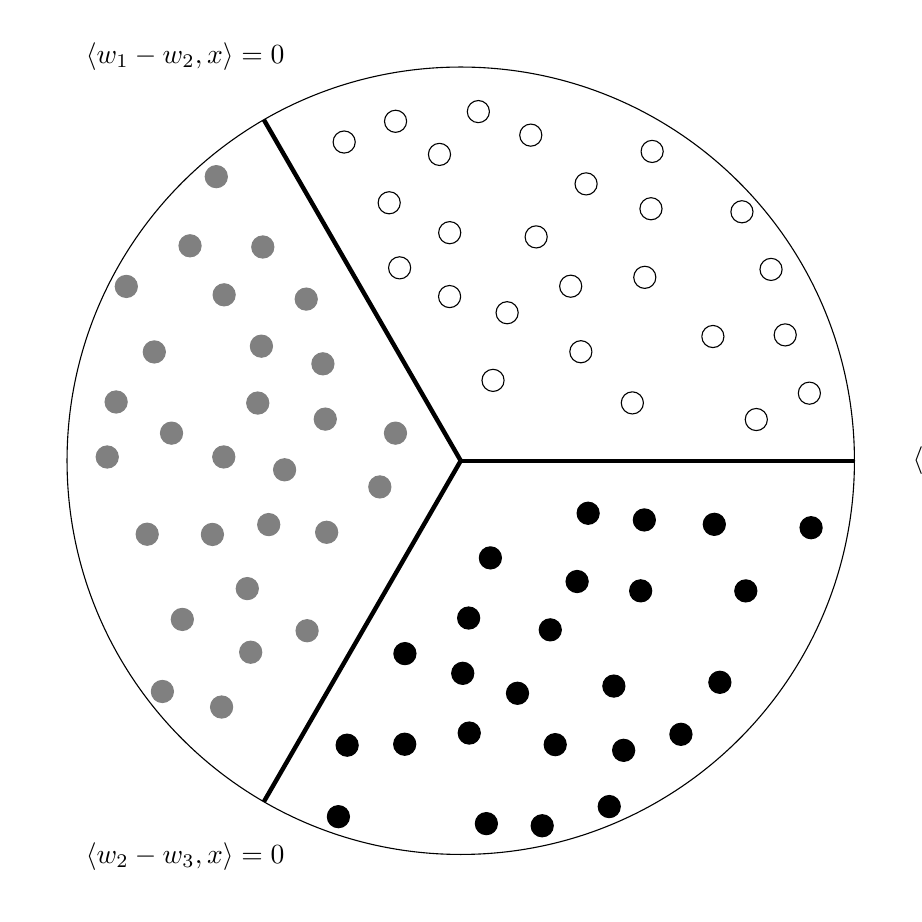
\begin{tikzpicture}

  \useasboundingbox (-5.5,-5.5) rectangle (5.5,5.5);
  % \draw[help lines] (-5.5,-5.5) rectangle (5.5,5.5);

  % Grid and coordinate axes
  %% \draw[help lines] (-5.2,-5.2) grid (5.2,5.2);
  %% \draw[thick, ->, >=latex] (-5.2,0) -- (5.2,0);
  %% \draw[thick, ->,  >=latex] (0,-5.2) -- (0,5.2);

  % Notable points
  \coordinate (Origin) at (0,0);

  \coordinate [label={[xshift=-10mm, yshift=5mm]$\ip{w_1 - w_2}{x} = 0$}] (A) at (120:5);
  \coordinate [label={[xshift=-10mm, yshift=-10mm]$\ip{w_2 - w_3}{x} = 0$}] (B) at (240:5);
  \coordinate [label={[xshift=+20mm, yshift=-3mm]$\ip{w_3 - w_1}{x} = 0$}] (C) at (360:5);

  % Circle which contains all the examples.
  \draw (Origin) circle (5);

  \draw[ultra thick] (Origin) -- (A);
  \draw[ultra thick] (Origin) -- (B);
  \draw[ultra thick] (Origin) -- (C);

  % Class 0 points. Angles between 0.0 and 120.0
  \draw[color=black, fill=none]
                    (7.94:3.79) circle (4pt)
                    (10.97:4.51) circle (4pt)
                    (18.63:2.30) circle (4pt)
                    (21.20:4.42) circle (4pt)
                    (26.23:3.57) circle (4pt)
                    (31.66:4.63) circle (4pt)
                    (41.52:4.77) circle (4pt)
                    (42.22:2.06) circle (4pt)
                    (44.90:3.30) circle (4pt)
                    (52.95:4.01) circle (4pt)
                    (57.79:2.62) circle (4pt)
                    (58.25:4.62) circle (4pt)
                    (65.64:3.86) circle (4pt)
                    (68.11:1.10) circle (4pt)
                    (71.38:3.00) circle (4pt)
                    (72.60:1.97) circle (4pt)
                    (77.86:4.23) circle (4pt)
                    (87.11:4.44) circle (4pt)
                    (92.77:2.90) circle (4pt)
                    (93.88:2.09) circle (4pt)
                    (93.97:3.90) circle (4pt)
                    (100.87:4.39) circle (4pt)
                    (105.50:3.40) circle (4pt)
                    (107.58:2.57) circle (4pt)
                    (110.09:4.31) circle (4pt)
                    ;

  % Class 1 points. Angles between 120.0 and 240.0
  \draw[color=gray, fill=gray]
                    (130.71:4.76) circle (4pt)
                    (132.80:3.70) circle (4pt)
                    (133.71:2.84) circle (4pt)
                    (141.55:4.39) circle (4pt)
                    (144.89:2.14) circle (4pt)
                    (144.96:3.67) circle (4pt)
                    (150.11:2.92) circle (4pt)
                    (152.47:4.79) circle (4pt)
                    (157.09:0.90) circle (4pt)
                    (160.45:4.13) circle (4pt)
                    (162.92:1.80) circle (4pt)
                    (164.13:2.68) circle (4pt)
                    (170.32:4.44) circle (4pt)
                    (174.55:3.69) circle (4pt)
                    (179.08:3.01) circle (4pt)
                    (179.39:4.49) circle (4pt)
                    (182.94:2.24) circle (4pt)
                    (193.19:4.09) circle (4pt)
                    (196.53:3.29) circle (4pt)
                    (197.93:1.08) circle (4pt)
                    (198.39:2.57) circle (4pt)
                    (208.08:1.93) circle (4pt)
                    (209.68:4.07) circle (4pt)
                    (210.92:3.16) circle (4pt)
                    (217.72:4.79) circle (4pt)
                    (222.35:3.61) circle (4pt)
                    (225.84:4.36) circle (4pt)
                    (227.89:2.91) circle (4pt)
                    ;

% Class 2 points. Angles between 240.0 and 360.0
  \draw[color=black, fill=black]
                    (248.23:3.89) circle (4pt)
                    (251.03:4.78) circle (4pt)
                    (253.86:2.55) circle (4pt)
                    (258.82:3.67) circle (4pt)
                    (270.54:2.70) circle (4pt)
                    (271.79:3.46) circle (4pt)
                    (272.88:2.00) circle (4pt)
                    (274.04:4.62) circle (4pt)
                    (282.58:4.75) circle (4pt)
                    (283.72:3.04) circle (4pt)
                    (286.97:1.29) circle (4pt)
                    (288.41:3.80) circle (4pt)
                    (293.24:4.78) circle (4pt)
                    (297.90:2.43) circle (4pt)
                    (299.36:4.22) circle (4pt)
                    (304.20:3.46) circle (4pt)
                    (308.83:4.46) circle (4pt)
                    (313.94:2.13) circle (4pt)
                    (319.47:4.33) circle (4pt)
                    (324.13:2.82) circle (4pt)
                    (335.46:3.98) circle (4pt)
                    (337.60:1.75) circle (4pt)
                    (342.13:2.45) circle (4pt)
                    (345.92:3.32) circle (4pt)
                    (349.18:4.53) circle (4pt)
                    ;

\end{tikzpicture}

\end{center}
\caption[]{The figure shows labeled examples in $\R^2$. The examples belong to
$K=3$ classes colored white, gray and black respectively. Each class lies in a
$120^\circ$ wedge. In other words, each class lies in an intersection of two
halfspaces.

While the examples are linearly separable with a positive margin $\gamma$, they
are \emph{not} strongly linearly separable with any positive margin $\gamma$.
}
\label{figure:linearly-separable-examples-with-margin}
\end{figure}


\section{Algorithm for strongly linearly separable data}
\label{section:algorithm-for-strongly-linearly-separable-data}

In this section, we present an algorithm for \textsc{Online Multiclass
Classification with Bandit Feedback} and prove an upper bound on the number of
mistakes under the assumption that the examples are strongly linearly separable
with a margin. The algorithm is stated as
Algorithm~\ref{algorithm:algorithm-for-strongly-linearly-separable-examples} and
the mistake upper bound is stated as
\autoref{theorem:strongly-separable-example-mistake-upper-bound}.

The idea behind the algorithm is to use $K$ copies of the \textsc{Binary
Perceptron} algorithm. Each copy corresponds to a class. In each round, each
copy makes a binary decision whether the feature vector belongs its respective
class or not. If at least one copy makes a positive prediction, the algorithm
predicts accordingly. If multiple copies make positive predictions, the
algorithm chooses one of them arbitrarily. If all copies make negative
predictions, the algorithms makes a blind guess.

\begin{algorithm}[h]
\caption{\textsc{Bandit Algorithm for Strongly Linearly Separable Examples}
\label{algorithm:algorithm-for-strongly-linearly-separable-examples}}
\begin{algorithmic}[1]
{
\REQUIRE{Number of classes $K$. Number of rounds $T$. Inner product space $(V,\ip{\cdot}{\cdot})$.}
\STATE{Initialize $w_1^{(1)} = w_2^{(1)} = \dots = w_K^{(1)} = 0$}
\FOR{$t=1,2,\dots,T$}
\STATE{Observe feature vector $x_t \in V$}
\STATE{Compute $S_t = \left\{ i ~:~ 1 \le i \le K, \ \ip{w_i^{(t)}}{x_t} \ge 0 \right\}$}
\IF{$S_t = \emptyset$}
\STATE{Predict $\widehat y_t \sim \text{Uniform}(\{1,2,\dots,K\})$}
\ELSE
\STATE{Predict $\widehat y_t \in S_t$ chosen arbitrarily}
\ENDIF
\STATE{Observe feedback $z_t \in \{0,1\}$ where $z_t = \indicator{\widehat y_t \neq y_t}$}
\IF{$S_t = \emptyset$}
\IF{$z_t = 1$}
\STATE{Set $w_i^{(t+1)} = w_i^{(t)}$ for all $i \in \{1,2,\dots,K\}$}
\ELSE
\STATE{Set $w_i^{(t+1)} = w_i^{(t)}$ for all $i \in \{1,2,\dots,K\} \setminus \{\widehat y_t\}$}
\STATE{Update $w_{\widehat y_t}^{(t+1)} = w_{\widehat y_t}^{(t)} + x_t$}
\ENDIF
\ELSE
\IF{$z_t = 1$}
\STATE{Set $w_i^{(t+1)} = w_i^{(t)}$ for all $i \in \{1,2,\dots,K\} \setminus \{\widehat y_t\}$}
\STATE{Update $w_{\widehat y_t}^{(t+1)} = w_{\widehat y_t}^{(t)} - x_t$}
\ELSE
\STATE{Set $w_i^{(t+1)} = w_i^{(t)}$ for all $i \in \{1,2,\dots,K\}$}
\ENDIF
\ENDIF
\ENDFOR
}
\end{algorithmic}
\end{algorithm}

\begin{theorem}[Mistake upper bound]
\label{theorem:strongly-separable-example-mistake-upper-bound}
Let $(V, \ip{\cdot}{\cdot})$ be any inner product space, let $K$ be a positive
integer, $\gamma$ a positive real number, $R$ be a non-negative real number. If
$(x_1, y_1), (x_2, y_2), \dots, (x_T, y_T)$ is a sequence of labeled examples in
$V \times \{1,2,\dots,K\}$ such that the examples are strongly separable with
margin $\gamma$ and $\norm{x_1}, \norm{x_2}, \dots, \norm{x_T} \le R$ then the
expected number of mistakes
Algorithm~\ref{algorithm:algorithm-for-strongly-linearly-separable-examples}
makes is at most $(K-1) \lfloor (R/\gamma)^2 \rfloor$.
\end{theorem}

\begin{proof}
Let $M = \sum_{t=1}^T z_t$ be the number of mistakes the algorithm makes. Let $A
= \sum_{t ~:~ S_t \neq \emptyset} z_t$ be the number of mistakes in the rounds
when $S_t \neq \emptyset$ and let $B = \sum_{t ~:~ S_t = \emptyset} z_t$ be the
number of mistakes in the rounds when $S_t = \emptyset$. Obviously, $M = A + B$.
We upper bound $A$ and $B$ separately.

Let $C$ be the number of times line 16 gets executed. Let $U$ be the number of
times line 16 and line 21 get executed. In other words, $U$ is the number of
times the $K$-tuple of vectors $(w_1^{(t)}, w_2^{(t)}, \dots, w_K^{(t)})$ gets
updated. Clearly, $U = A + C$.

The key observation is that $\Exp[B] = (K-1) \Exp[C]$ since if $S_t =
\emptyset$, there is $1/K$ probability that the algorithm guesses the correct
label and with probability $(K-1)/K$ algorithm's guess is incorrect.
Putting all the information together, we get that
\begin{align*}
\Exp[M]
& = \Exp[A] + \Exp[B] \\
& = \Exp[A] + (K-1) \Exp[C]  \\
& \le (K-1) \Exp[A + C] \\
& = (K-1) \Exp[U]  \; .
\end{align*}

To finish the proof, we need to upper bound the number of updates, $U$. We claim
that $U \le \lfloor (R/\gamma)^2 \rfloor$. The proof of this upper bound is
similar to the proof of the mistake bound for \textsc{Multiclass Perceptron}
algorithm. Let $w_1^*, w_2^*, \dots, w_K^* \in V$ be vectors that satisfy
\eqref{equation:strong-linear-separability-1},
\eqref{equation:strong-linear-separability-2} and
\eqref{equation:strong-linear-separability-3}.
The $K$-tuple $(w_1^{(t)}, w_2^{(t)}, \dots, w_K^{(t)})$
changes only if there is an update in round $t$.
We investigate how $\sum_{i=1}^K \norm{w_i^{(t)}}^2$ and
$\sum_{i=1}^K \ip{w_i^*}{w_i^{(t)}}$ change. If there is an update in round $t$,
we have
\begin{align*}
\sum_{i=1}^K \norm{w_i^{(t+1)}}^2
& = \left( \sum_{i \in \{1,2,\dots,K\} \setminus \{\widehat y_t\}} \norm{w_i^{(t)}}^2 \right) + \norm{w_{\widehat y_t}^{(t+1)}}^2 \\
& = \left( \sum_{i \in \{1,2,\dots,K\} \setminus \{\widehat y_t\}} \norm{w_i^{(t)}}^2 \right) + \norm{w_{\widehat y_t}^{(t)} + (-1)^{z_t} x_t}^2 \\
& = \left( \sum_{i=1}^K \norm{w_i^{(t)}}^2 \right) + \norm{x_t}^2 + \underbrace{(-1)^{z_t} 2 \ip{w_{\widehat y_t}^{(t)}}{x_t}}_{\le 0} \\
& \le \left( \sum_{i=1}^K \norm{w_i^{(t)}}^2 \right) + \norm{x_t}^2 \\
& \le \left( \sum_{i=1}^K \norm{w_i^{(t)}}^2 \right) + R^2 \; .
\end{align*}
Therefore, after $U$ updates,
$$
\sum_{i=1}^K \norm{w_i^{(T+1)}}^2 \le R^2 U \; .
$$
Similarly, if there is an update in round $t$, we have
\begin{align*}
\sum_{i=1}^K \ip{w_i^*}{w_i^{(t)}}
& = \left( \sum_{i \in \{1,2,\dots,K\} \setminus \{\widehat y_t\}} \ip{w_i^*}{w_i^{(t)}} \right) + \ip{w_{\widehat y_t}^*}{w_{\widehat y_t}^{(t+1)}} \\
& = \left( \sum_{i \in \{1,2,\dots,K\} \setminus \{\widehat y_t\}} \ip{w_i^*}{w_i^{(t)}} \right) + \ip{w_{\widehat y_t}^*}{w_{\widehat y_t}^{(t)} + (-1)^{z_t} x_t} \\
& = \left( \sum_{i=1}^K \ip{w_i^*}{w_i^{(t)}} \right) + (-1)^{z_t} \ip{w_{\widehat y_t}^*}{x_t} \\
& \ge \left( \sum_{i=1}^K \ip{w_i^*}{w_i^{(t)}} \right) + \gamma
\end{align*}
where the last inequality follows from \eqref{equation:strong-linear-separability-2}
and \eqref{equation:strong-linear-separability-3} and case analysis whether $z_t = 0$ or $z_t = 1$.
Thus, after $U$ updates,
$$
\sum_{i=1}^K \ip{w_i^*}{w_i^{(T+1)}} \ge \gamma U \; .
$$
Applying Cauchy-Schwartz's inequality twice and assumption
\eqref{equation:strong-linear-separability-1}, we get that
$$
\sum_{i=1}^K \ip{w_i^*}{w_i^{(T+1)}}
\le \sum_{i=1}^K \norm{w_i^*} \cdot \norm{w_i^{(T+1)}}
\le \sqrt{\sum_{i=1}^K \norm{w_i^*}^2} \sqrt{\sum_{i=1}^K \norm{w_i^{(T+1)}}^2}
\le \sqrt{\sum_{i=1}^K \norm{w_i^{(T+1)}}^2} \; .
$$
Combining the upper and lower bounds on $\sum_{i=1}^K \norm{w_i^{(T+1)}}^2$ inequalities, we get
$$
(\gamma U)^2 \le \sum_{i=1}^K \norm{w_i^{(T+1)}}^2 \le R^2 U \; .
$$
We conclude that $U \le (R/\gamma)^2$. Since $U$ is an integer, $U \le \lfloor (R/\gamma)^2 \rfloor$.
\end{proof}

\begin{theorem}[Mistake lower bound]
\label{theorem:strongly-separable-example-mistake-lower-bound}
Let $\gamma$ be a positive real number and let $R$ be a non-negative real
number. For any (possibly randomized) algorithm for the \textsc{Online
Multiclass Classification with Bandit Feedback} with $K \le
\frac{1}{4}(R/\gamma)^2$ classes there exists an inner product space $(V,
\ip{\cdot}{\cdot})$, a non-negative integer $T$ and a sequence of labeled
examples $(x_1, y_1), (x_2, y_2), \dots, (x_T, y_T)$ in $V \times
\{1,2,\dots,K\}$ that are strongly linearly separable with margin $\gamma$, the
norms satisfy $\norm{x_1}, \norm{x_2}, \dots, \norm{x_T} \le R$ and the expected
number of mistakes the algorithm makes is at least $\frac{K-1}{2} \lfloor
\frac{1}{16} (R/\gamma)^2 \rfloor$.
\end{theorem}

\begin{proof}
We use probabilistic method. Let $M = \lfloor \frac{1}{16} (R/\gamma)^2 \rfloor$.
Let $V = \R^{M+1}$ equipped with the standard inner product.  Let $e_1, e_2,
\dots, e_{M+1}$ be the standard orthonormal basis of $V$. We define
vectors $v_1, v_2, \dots, v_M \in V$ where $v_i = \frac{R}{\sqrt{2}}(e_i +
e_{M+1})$ for $i=1,2,\dots,M$. Let $\ell_1, \ell_2, \dots, \ell_M$ be chosen
i.i.d. uniformly at random from $\{1,2,\dots,K\}$ and independently of any
randomness used the by the algorithm. Let $T = M K$. We define examples $(x_1,
y_1), (x_2, y_2), \dots, (x_T, y_T)$ as follows:
$$
\begin{array}{lclclclcl}
(x_1, y_1) & = & (x_2, y_2) & = & \cdots & = & (x_K, y_K) & = & (v_1, \ell_1) \; , \\
(x_{K+1},y_{K+1}) & = & (x_{K+2}, y_{K+2}) & = & \cdots & = & (x_{2K}, y_{2K}) & = & (v_2, \ell_2) \; , \\
& \vdots & \\
(x_{(M-1)K+1}, y_{(M-1)K+1})  & = & (x_{(M-1)K+2}, y_{(M-1)K+2}) & = & \cdots & = & (x_{MK}, y_{MK}) & = & (v_M, \ell_M) \; .
\end{array}
$$

With probability one, norm of each example is $R$. We show that with probability
one, the examples are strongly separable with margin $\gamma$. In order to see
that consider $w_1^*, w_2^*, \dots, w_K^* \in V$ defined by
$$
w_i^* = 2 \sqrt{2} \frac{\gamma}{R} \left( \sum_{j ~:~ \ell_j = i} e_j \right) - \sqrt{2} \frac{\gamma}{R} e_{M+1} \qquad \quad \text{for $i=1,2,\dots,K$.}
$$
Since for any $i \in \{1,2,\dots,K\}$ and any $j \in \{1,2,\dots,M\}$,
$$
\ip{w_i^*}{v_j} =
\begin{cases}
\gamma & \text{if $\ell_j = i$,} \\
- \gamma & \text{if $\ell_j \neq i$,}
\end{cases}
$$
it means that $w_1^*, w_2^*, \dots, w_K^*$ satisfy
\eqref{equation:strong-linear-separability-2} and
\eqref{equation:strong-linear-separability-3}. Condition \eqref{equation:strong-linear-separability-1}
is satisfied since
$$
\sum_{i=1}^K \norm{w_i^*}^2
= 8 \frac{\gamma^2}{R^2} \sum_{j=1}^M \norm{e_j}^2 + 2 \frac{\gamma^2}{R^2} K \norm{e_{M+1}}^2
= 8 \frac{\gamma^2}{R^2} M + 2 \frac{\gamma^2}{R^2} K
\le \frac{1}{2} + \frac{1}{2}
= 1 \; .
$$

It remains to lower bound the expected number of mistakes of the algorithm. For
any $j \in \{1,2,\dots,M\}$, consider the expected number of mistakes the
algorithm makes in rounds $K(j-1) + 1, K(j-1) + 2, \dots, Kj$. In these rounds,
the algorithm is guessing the label $\ell_j$. Since $\ell_j$ is chosen uniformly
at random from the set $\{1,2,\dots,K\}$ and feedback is only binary, the
expected number of mistakes the algorithm makes in these rounds is at least
$\frac{K-1}{2}$. Altogether, the algorithm makes at least $\frac{K-1}{2} M$
mistakes in expectation.

Finally, since strong separability and norm condition hold with probability one,
there exists a particular (i.e. deterministic) sequence of examples for which
the algorithm makes at least $\frac{K-1}{2} M$ mistakes in expectation
over its internal randomization.
\end{proof}

\section{Converting linear separability to strong linear separability}
\label{section:converting-linear-separability-to-strong-linear-separability}

In this section, we show how construct a mapping $\phi$ of points in the unit
ball of $\R^d$ into a high dimensional inner product space that has the
property if any set of labeled examples in the unit ball is linearly separable with a
margin $\gamma$, applying the mapping $\phi$ makes the examples \emph{strongly}
linearly separable with a margin $\gamma'$ and their norms are bounded by $R'$.
The parameters $\gamma'$ and $R'$ are functions of the old margin $\gamma$ and
the number of classes $K$, and the are specified in the theorems below.

Equipped with the mapping $\phi$, we can utilize
Algorithm~\ref{algorithm:algorithm-for-strongly-linearly-separable-examples} and
\autoref{theorem:strongly-separable-example-mistake-upper-bound} from the
previous section and we obtain an algorithm for linearly separable examples and
an upper bound on its number of mistakes. As a computational speed up, instead
of working with the mapped examples $\phi(x_1), \phi(x_2), \dots$ explicitly, we
can use the kernelized version of
Algorithm~\ref{algorithm:algorithm-for-strongly-linearly-separable-examples}
that uses a kernel function $k(x,x') = \ip{\phi(x)}{\phi(x')}$.

We construct several different mappings $\phi$. The parameters $R'$ and
$\gamma'$ for the different mappings are not the same, but the ratios
$R'/\gamma'$ are qualitively the same. However, one mapping has the advantage of
having a kernel $k(x,x')$ that is faster to evaluate. Another mapping has the
advantage that one does \emph{not} need to know the initial margin $\gamma$. In
other words, the same mapping works for all possible values of $\gamma > 0$.

The idea behind all the mappings is that, on a compact set, multivariate
polynomials uniformly approximate any continuous function. This result is a
special case of the well known Stone-Weierstrass theorem; see
e.g.~\citep[Section~10.10]{Davidson-Donsig-2010}. In our case, we use
multivariate polynomial to approximate the indicator function corresponding to
the intersection of $K-1$ halfspaces. This polynomial separates examples in one
class from examples in the other classes. To be able to quantify $\gamma'$ and
$R'$ as well as time complexity of evaluating $k(x,x')$ we need to quantify
certain parameters of the approximating polynomial (degree, norm, range of
values). We construct two different polynomials with different paremeters. The
parameters are quantified in
Theorems~\ref{theorem:polynomial-approximation-1}~and~\ref{theorem:polynomial-approximation-2}
stated below.

Before we state the theorems, recall that a polynomial of $d$ variables is a
function $p:\R^d \to \R$ of the form
$$
p(x) = p(x_1, x_2, \dots, x_d) = \sum_{i_1, i_2, \dots, i_d} c_{i_1, i_2, \dots, i_d} x_1^{i_1} x_2^{i_2} \dots x_d^{i_d}
$$
where the sum ranges over a finite set of $d$-tuples $(i_1, i_2, \dots, i_d)$ of
non-negative integers and $c_{i_1, i_2, \dots, i_d}$ is a real coefficient. The
\emph{degree} of a polynomial $p$, denoted by $\deg(p)$, is the largest value of
$i_1 + i_2 + \dots + i_d$ for which the coefficient is non-zero. The \emph{norm
of a polynomial} $p$ is defined as
$$
\norm{p} = \sqrt{\sum_{i_1, i_2, \dots, i_d} \left(c_{i_1, i_2, \dots, i_d} \right)^2 } \; .
$$
It is not hard to see that this indeed a norm, since we can interpret it as
a Euclidean norm of the vector of the coefficients of the polynomial.

\begin{theorem}[Polynomial approximation of intersection of halfspaces I]
\label{theorem:polynomial-approximation-1}
Let $v_1, v_2, \dots, v_m \in \R^d$ be vectors such that $\norm{v_1}, \norm{v_2}, \dots, \norm{v_m} \le 1$.
Let $\gamma > 0$. There exists a polynomial $p:\R^d \to \R$ such that
\begin{enumerate}
\item $p(x) \ge 1$ for all $x \in \bigcap_{i=1}^m \left\{ x \in \R^d ~:~ \norm{x} \le 1, \ \ip{v_i}{x} \ge \gamma \right\}$
\item $p(x) \le -1$ for all $x \in \bigcup_{i=1}^m \left\{ x \in \R^d ~:~ \norm{x} \le 1, \ \ip{v_i}{x} \le - \gamma \right\}$
\item $\deg(p) \le ???$
\item $\norm{p} \le ???$
\item $|p(x)| \le ???$ for all $x \in \R^d$ such that $\norm{x} \le 1$
\end{enumerate}
\end{theorem}

\begin{theorem}[Polynomial approximation of intersection of halfspaces II]
\label{theorem:polynomial-approximation-2}
Let $v_1, v_2, \dots, v_m \in \R^d$ be vectors such that $\norm{v_1}, \norm{v_2}, \dots, \norm{v_m} \le 1$.
Let $\gamma > 0$. There exists a polynomial $p:\R^d \to \R$ such that
\begin{enumerate}
\item $p(x) \ge 1/2$ for all $x \in \bigcap_{i=1}^m \left\{ x \in \R^d ~:~ \norm{x} \le 1, \ \ip{v_i}{x} \ge \gamma \right\}$
\item $p(x) \le -1/2$ for all $x \in \bigcup_{i=1}^m \left\{ x \in \R^d ~:~ \norm{x} \le 1, \ \ip{v_i}{x} \le - \gamma \right\}$
\item $\deg(p) \le ???$
\item $\norm{p} \le ???$
\item $|p(x)| \le ???$ for all $x \in \R^d$ such that $\norm{x} \le 1$
\end{enumerate}
\end{theorem}

The proofs of the theorems can be found in
Sections~\ref{section:proof-of-polynomial-approximation-1}~and~\ref{section:proof-of-polynomial-approximation-2}
respectively.

\subsection{Proof of \autoref{theorem:polynomial-approximation-1}}
\label{section:proof-of-polynomial-approximation-1}

\begin{lemma}[Inequality]
\label{lemma:inequality}
For any real numbers $b_1, b_2, \dots, b_n$,
$$
\left( \sum_{i=1}^n b_i \right)^2 \le n \sum_{i=1}^n b_i^2 \; .
$$
\end{lemma}

\autoref{lemma:inequality} follows from Cauchy-Schwartz inequality applied to
vectors $(b_1, b_2, \dots, b_n)$ and $(1,1,\dots,1)$.

\begin{proposition}[Properties of the norm of polynomials]
\hspace{1cm} % Dummy space
\begin{enumerate}
\item Let $p_1, p_2, \dots, p_n$ be multivariate polynomials and
let $p(x) = \prod_{j=1}^n p_j(x)$ be their product. Then, $\norm{p}^2 \le n^{\sum_{j=1}^n \deg(p_j)} \prod_{j=1}^n \norm{p_j}^2$.
\item Let $q$ be a multivariate polynomial of degree at most $s$ and let $p(x) = (q(x))^n$. Then, $\norm{p}^2 \le n^{ns} \norm{q}^{2n}$.
\item Let be $p_1, p_2, \dots, p_n$ be multivariate polynomials. Then, $\norm{\sum_{j=1}^n p_j}^2 \le n \sum_{j=1}^n \norm{p_j}^2$.
\end{enumerate}
\end{proposition}

\begin{proof}
Using multi-index notation we can write any multivariate polynomial $p$ as
$$
p(x) = \sum_A c_A x^A
$$
where $A = (i_1, i_2, \dots, i_d)$ is a multi-index (i.e. a $d$-tuple of
non-negative integers), $x^A = x_1^{i_1} x_2^{i_2} \dots x_d^{i_d}$ is a
monomial and $c_A = c_{i_1, i_2, \dots, i_d}$ is the corresponding real
coefficient. The sum is over a finite subset of $d$-tuples of non-negative
integers. Using this notation, the norm of a polynomial $p$ can be written as
$$
\norm{p} = \sqrt{\sum_A (c_A)^2} \; .
$$
For a multi-index $A = (i_1, i_2, \dots, i_d)$ we define its $1$-norm as
$\norm{A}_1 = i_1 + i_2 + \dots + i_d$.

To prove the first part, we express $p_j$ as
$$
p_j(x) = \sum_{A_j} c^{(j)}_{A_j} x^{A_j} \; .
$$
If $p$ has expansion $p(x) = \sum_A c_A x^A$ then its coefficient $c_A$ for any multi-index $A$ is
$$
c_A = \sum_{\substack{(A_1, A_2, \dots, A_n) \\ A_1 + A_2 + \dots + A_n = A}} c^{(1)}_{A_1} c^{(2)}_{A_2} \cdots c^{(n)}_{A_n} \; .
$$
Therefore,
\begin{multline*}
\norm{p}^2
= \sum_{A} (c_A)^2
= \sum_{A} \left( \sum_{\substack{(A_1, A_2, \dots, A_n) \\ A_1 + A_2 + \dots + A_n = A}} c^{(1)}_{A_1} c^{(2)}_{A_2} \cdots c^{(n)}_{A_n} \right)^2
= \sum_{A} \left( \sum_{\substack{(A_1, A_2, \dots, A_n) \\ A_1 + A_2 + \dots + A_n = A}} \prod_{j=1}^n c^{(j)}_{A_j} \right)^2
\end{multline*}
and
\begin{multline*}
\prod_{i=1}^n \norm{p_i}^2
= \prod_{i=1}^n \left( \sum_{A_i} (c^{(i)}_{A_i})^2 \right)
= \sum_{(A_1, A_2, \dots, A_n)} \prod_{j=1}^n (c^{(j)}_{A_j})^2
= \sum_{(A_1, A_2, \dots, A_n)} \left( \prod_{j=1}^n c^{(j)}_{A_j} \right)^2 \\
= \sum_A \sum_{\substack{(A_1, A_2, \dots, A_n) \\ A_1 + A_2 + \dots + A_n = A}} \left( \prod_{j=1}^n c^{(j)}_{A_j} \right)^2
\end{multline*}
where in both cases the outer sum is over multi-indices $A$ such that $\norm{A}_1 \le \deg(p)$.
To finish the proof, it is sufficient to prove that for any $A$ such that $\norm{A}_1 \le \deg(p)$,
$$
\left( \sum_{\substack{(A_1, A_2, \dots, A_n) \\ A_1 + A_2 + \dots + A_n = A}} \prod_{j=1}^n c^{(j)}_{A_j} \right)^2
\le n^{\deg(p)} \sum_{\substack{(A_1, A_2, \dots, A_n) \\ A_1 + A_2 + \dots + A_n = A}} \left( \prod_{j=1}^n c^{(j)}_{A_j} \right)^2 \; .
$$
This inequality follows from \autoref{lemma:inequality} as long we can show that
the number of $n$-tuples $(A_1, A_2, \dots, A_n)$ such that $A_1 + A_2 + \dots +
A_n = A$ is upper bounded by $n^{\deg(p)}$.

The second part follows from the first part by setting $p_1 = p_2 = \dots p_n = q$.

To prove the third part we use generalized triangle inequality and an
\autoref{lemma:inequality}. We have
\begin{align*}
\norm{\sum_{j=1}^n p_j}^2 = \left( \norm{\sum_{j=1}^n p_j} \right)^2 \le \left(\sum_{j=1}^n \norm{p_j} \right)^2 \le n \sum_{j=1}^n \norm{p_j}^2 \; .
\end{align*}
\end{proof}

\subsection{Proof of \autoref{theorem:polynomial-approximation-2}}
\label{section:proof-of-polynomial-approximation-2}

To construct the polynomial $p$ we use Chebyshev polynomials of the first kind.
Chebyshev polynomials of the fist kind form an infinite sequence of polynomials
$T_0(z), T_1(z), T_2(z), \dots$ of single real variable $z$. They are defined
by the recurrence
\begin{align*}
T_0(z) & = 1 \; , \\
T_1(z) & = z \; , \\
T_{n+1}(z) & = 2zT_n(z) - T_{n-1}(z) & \text{for $n \ge 1$.}
\end{align*}
Chebyshev polynomials have a lot of interesting properties.
We will need properties listed in
\autoref{proposition:properties-of-chebyshev-polynomials} below.
Interested reader can learn more about Chebyshev polynomials
from the book by \cite{Mason-Handscomb-2002}.

\begin{proposition}[Properties of Chebyshev polynomials]
\label{proposition:properties-of-chebyshev-polynomials}
Chebyshev polynomials satisfy
\begin{enumerate}
\item $\deg(T_n) = n$ for all $n \ge 0$.
\item If $n \ge 1$, the leading coefficient of $T_n(z)$ is $2^{n-1}$.
\item $|T_n(z)| \le 1$ for all $z \in [-1,1]$ and all $n \ge 0$.
\item $T_n(z) \ge 1 + n^2(z - 1)$ for all $z \ge 1$ and all $n \ge 0$.
\item All coefficients of $T_n(z)$ lie in the interval $\left[-(1+\sqrt{2})^n, (1+\sqrt{2})^n \right]$.
\end{enumerate}
\end{proposition}

\begin{proof}[Proof of \autoref{proposition:properties-of-chebyshev-polynomials}]
The first two proprties easily follow from the recurrence.

The third property is a direct consequence of
\begin{equation}
\label{equation:trigonometric-chebyshev}
T_n(\cos(\theta)) = \cos(n \theta) \qquad \quad \text{for all $\theta \in \R$.}
\end{equation}
since for any $x \in [-1,1]$ there exists $\theta \in \R$ such that $\cos(\theta) = x$.
Equation \eqref{equation:trigonometric-chebyshev} is proved by induction on $n$. Indeed, by definition
$$
T_0(\cos(\theta)) = 1 = \cos(0 \theta) \qquad \text{and} \qquad T_1(\cos(\theta)) = \cos(\theta) \; .
$$
For $n \ge 1$, we have
\begin{align*}
T_{n+1}(\cos(\theta))
& = 2 \cos(\theta) T_n(\cos(\theta)) - T_{n-1}(\cos(\theta)) \\
& = 2 \cos(\theta) \cos(n \theta) - \cos((n-1)\theta)) \; ,
\end{align*}
where the last step follow by induction hypothesis.
It remains to show that the last expression equals $\cos((n+1)\theta)$.
This can be derived from the trigonometric formula
$$
\cos(\alpha \pm \beta) = \cos(\alpha) \cos(\beta) \mp \sin(\alpha) \sin(\beta) \; .
$$
By substituting $\alpha = n \theta$ and $\beta = \theta$, we get two equations
\begin{align*}
\cos((n+1) \theta) & = \cos(n \theta) \cos(\theta) - \sin(n \theta) \sin(\theta) \; , \\
\cos((n-1) \theta) & = \cos(n \theta) \cos(\theta) + \sin(n \theta) \sin(\theta) \; .
\end{align*}
Summing them yields
$$
\cos((n+1)\theta) + \cos((n-1) \theta) = 2 \cos(n \theta) \cos(\theta)
$$
which finishes the proof of equation \eqref{equation:trigonometric-chebyshev}.

To verify the fourth property we first show that
\begin{equation}
\label{equation:hyperbolic-chebyshev}
T_n(\cosh(\theta)) = \cosh(n \theta) \qquad \quad \text{for all $\theta \in \R$.}
\end{equation}
The proof of equation~\eqref{equation:hyperbolic-chebyshev} is the same
as the proof of equation \eqref{equation:trigonometric-chebyshev} except
that we replace $\cos$ and $\sin$ with $\cosh$ and $\sinh$ respectively.

Note that $\cosh(\theta) = \frac{e^{\theta} + e^{-\theta}}{2}$ is an even
continuous function that maps $\R$ onto $[1,+\infty)$, is strictly decreasing
on $(-\infty,0]$, and is strictly increasing on $[0,\infty)$. Thus the fourth
property is equivalent to
$$
T_n(\cosh(\theta)) \ge 1 + n^2 (\cosh(\theta) - 1) \qquad \text{for all $\theta \ge 0$.}
$$
For $\theta = 0$, according to \eqref{equation:hyperbolic-chebyshev} both sides
are equal to $1$. Thus, it is sufficient to prove that the derivative of the
left hand side is greater or equal to the derivative of the right hand side.
That is, we need to prove that
\begin{equation}
\label{equation:hyperbolic-chebyshev-derivative-inequality}
\frac{\diff T_n(\cosh(\theta))}{\diff \theta} \ge \frac{\diff (1 + n^2 (\cosh(\theta) - 1))}{\diff \theta} \qquad \text{for all $\theta \ge 0$.}
\end{equation}
Using \eqref{equation:hyperbolic-chebyshev} and recalling that $\frac{\diff \cosh(\theta)}{\diff \theta} = \sinh(\theta)$ we
can express the derivatives as
\begin{align*}
\frac{\diff T_n(\cosh(\theta))}{\diff \theta} & = \frac{\diff \cosh(n \theta))}{\diff \theta} = n \sinh(n \theta) \; , \\
\frac{\diff (1 + n^2 (\cosh(\theta) - 1))}{\diff \theta} & = n^2 \sinh(\theta) \; .
\end{align*}
The inequality \eqref{equation:hyperbolic-chebyshev-derivative-inequality} is thus equivalent to
$$
\sinh(n \theta) \ge n \sinh(\theta) \qquad \text{for all $\theta \ge 0$.}
$$
Tho prove this inequality we use the summation formula
$$
\sinh(\alpha + \beta) = \sinh(\alpha) \cosh(\beta) + \sinh(\beta) \cosh(\beta)
$$
and the observation that for $\theta \ge 0$, $\cosh(\theta) \ge 1$ and $\sinh(\theta) \ge 0$. Thus,
$$
\sinh(\alpha + \beta) \ge \sinh(\alpha) + \sinh(\beta) \qquad \text{for $\alpha, \beta \ge 0$.}
$$
Thus by induction on $n$, we see that $\sinh(n \theta) \ge n \sinh(\theta)$ for all $\theta \ge 0$.

To verify the fifth property let $a_n$ be the magnitude of the largest
coefficient of $T_n(z)$. The recurrence for Chebyshev polynomials
implies that the sequence $a_0, a_1, a_2, \dots$ satisfies
\begin{align*}
a_0 & = a_1 = 1 \; , \\
a_{n+1} & \le 2 a_n + a_{n-1} & \text{for $n \ge 1$.}
\end{align*}
It remains to show that $a_n \le (1 + \sqrt{2})^n$ for all $n \ge 0$. We do this
by induction on $n$. For $n=0$ and $n=1$ the inequality trivially holds. For $n
\ge 1$, we have
\begin{align*}
a_{n+1} \le 2 a_n + a_{n-1}
& \le 2 (1 + \sqrt{2})^n + (1 + \sqrt{2})^{n-1} \\
& = (1 + \sqrt{2})^{n-1} (2 (1 + \sqrt{2}) + 1) \\
& = (1 + \sqrt{2})^{n-1} (3 + 2\sqrt{2}) \\
& = (1 + \sqrt{2})^{n-1} (1 + \sqrt{2})^2 \\
& = (1 + \sqrt{2})^{n+1} \; .
\end{align*}

\end{proof}

Let $r = \left\lceil \log_2(2m) \right\rceil$ and $s = \left\lceil \sqrt{\frac{1}{\gamma}} \right\rceil$.
We define the polynomial $p:\R^d \to \R$ as
$$
p(x) = m + \frac{1}{2} - \sum_{i=1}^m \left( T_s(1 - \ip{v_i}{x}) \right)^r \; .
$$
It remains to show that $p$ has properties 1--5.


\subsection{Rational Kernel}
TODO

\section{Nearest neighbor algorithm}

TODO


\section{NP-hardness of the weak labeling problem}

Any algorithm for the bandit setting collects information in the form of so
called \emph{strongly labeled} and \emph{weakly labeled} examples.
Strongly-labeled examples are those for which we know the class label. Weakly
labeled example is an example for which we know that class label can be anything
except for a particular one class.

A natural strategy for each round is to find vectors $w_1, w_2, \dots, w_K$ that
linearly separate the examples seen in the previous rounds and use the vectors
to predict the label in the next round. More precisely, we want to find both the
vectors $w_1, w_2, \dots, w_K$ and label for each example consistent with its
weak and/or strong labels such that $w_1, w_2, \dots, w_K$ linearly separate the
labeled examples. We show this problem is NP-hard even for $K=3$.

Clearly, the problem is at least as hard as the decision version of the problem
where the goal is to determine if such vectors and labeling exist. We show that
this problem is NP-complete.

Formally, the input to the decision problem are positive integers $d, T, K$ and
a sequence $(x_1, y_1), (x_2, y_2), \dots, (x_T, y_T) \in \{0,1\}^d \times
\{1,2,\dots,K, \overline{1}, \overline{2}, \dots, \overline{K}\}$ of strongly
and weakly labeled examples. The numbers $1,2,\dots,K$ correspond to strong
labels and the symbols $\overline{1}, \overline{2}, \dots, \overline{K}$
correspond to weak labels. We adopt the convention that $\overline{\overline{i}}
= i$ for any positive integer $i$. The goal is to determine whether or not there
exist vectors $w_1, w_2, \dots, w_K \in \R^d$ that satisfy the following
conditions for all $t=1,2,\dots,T$,
\begin{align*}
y_t \in \{1,2,\dots,K\} \qquad & \Longrightarrow \qquad & \forall i \in \{1,2,\dots,K\} \setminus \{y_t\} \qquad \ip{w_{y_t}}{x_t} & > \ip{w_i}{x_t} \; , \\
y_t \in \{\overline{1}, \overline{2},\dots, \overline{K}\} \qquad & \Longrightarrow & \qquad \exists i \in \{1,2,\dots,K\} \qquad \ip{w_i}{x_t} & > \ip{w_{\overline{y_t}}}{x_t} \; .
\end{align*}

TODO

\section{Mistake lower bound for ignorant algorithms}

TODO

\bibliographystyle{plainnat}
\bibliography{biblio}

\appendix

\section{Multiclass Perceptron}
\label{section:multiclass-perceptron-proofs}

\textsc{Multiclass Perceptron} is an algorithm for \textsc{Online Multiclass
Classification}. Both the protocol for the problem and the algorithm are stated
below. The algorithm assumes that the feature vectors come from an inner product
space $(V, \ip{\cdot}{\cdot})$.

Two results are folklore. The first result is
\autoref{theorem:mutliclass-perceptron-mistake-upper-bound} which states that if
examples are linearly separable with margin $\gamma$ and examples have norm
at most $R$ then the algorithm makes at most $\lfloor 2 (R/\gamma)^2 \rfloor$
mistakes. The second result is
\autoref{theorem:online-multiclass-classification-mistake-lower-bound} which
states that under the same assumptions as in
\autoref{theorem:online-multiclass-classification-mistake-lower-bound}
\emph{any} deterministic algorithm for \textsc{Online Multiclass Classification}
must make at least $\lfloor (R/\gamma)^2 \rfloor$ mistakes in the worst case.

\begin{algorithm}[h]
\caption{\textsc{Online Multiclass Classification}
\label{algorithm:mutliclass-classification}}
\begin{algorithmic}[1]
{
\REQUIRE{Number of classes $K$. Number of rounds $T$.}
\FOR{$t=1,2,\dots,T$}
\STATE{Observe feature vector $x_t$}
\STATE{Predict $\widehat y_t \in \{1,2,\dots,K\}$}
\STATE{Observe $y_t \in \{1,2,\dots,K\}$}
\ENDFOR
}
\end{algorithmic}
\end{algorithm}

\begin{algorithm}[h]
\caption{\textsc{Multiclass Perceptron}
\label{algorithm:mutliclass-perceptron}}
\begin{algorithmic}[1]
{
\REQUIRE{Number of classes $K$. Number of rounds $T$. Inner product space $(V,\ip{\cdot}{\cdot})$.}
\STATE{Initialize $w_1^{(1)} = w_2^{(1)} = \dots = w_K^{(1)} = 0$}
\FOR{$t=1,2,\dots,T$}
\STATE{Observe feature vector $x_t \in V$}
\STATE{Predict $\widehat y_t = \argmax_{i \in \{1,2,\dots,K\}} \ip{w_t^{(i)}}{x_t}$}
\STATE{Observe $y_t \in \{1,2,\dots,K\}$}
\IF{$\widehat y_t \neq y_t$}
\STATE{Set $w_i^{(t+1)} = w_i^{(t)}$ for all $i \in \{1,2,\dots,K\} \setminus \{y_t, \widehat y_t\}$}
\STATE{Update $w_{y_t}^{(t+1)} = w_{y_t}^{(t)} + x_t$}
\STATE{Update $w_{\widehat y_t}^{(t+1)} = w_{\widehat y_t}^{(t)} - x_t$}
\ELSE
\STATE{Set $w_i^{(t+1)} = w_i^{(t)}$ for all $i \in \{1,2,\dots,K\}$}
\ENDIF
\ENDFOR
}
\end{algorithmic}
\end{algorithm}

\begin{theorem}[Mistake upper bound]
\label{theorem:mutliclass-perceptron-mistake-upper-bound}
Let $(V, \ip{\cdot}{\cdot})$ be an inner product space, let $K$ be a positive
integer, let $\gamma$ be a positive real number and let $R$ be a non-negative real
number. If $(x_1, y_1), (x_2, y_2), \dots, (x_T, y_T)$ is a sequence of labeled
examples in $V \times \{1,2,\dots,K\}$ that are linearly separable with margin
$\gamma$ and $\norm{x_1}, \norm{x_2}, \dots, \norm{x_T} \le R$
then \textsc{Multiclass Perceptron} algorithm makes at most $\lfloor
2(R/\gamma)^2 \rfloor$ mistakes.
\end{theorem}

\begin{proof}
Let $M = \sum_{t=1}^T \indicator{\widehat y_t \neq y_t}$ be the number of
mistakes the algorithm makes. Since the $K$-tuple $(w_1^{(t)}, w_2^{(t)}, \dots,
w_K^{(t)})$ changes only if a mistake is made, we can upper bound $\sum_{i=1}^K
\norm{w_i^{(t)}}^2$ in terms of number of mistakes.
If a mistake happens in round $t$,
\begin{align*}
\sum_{i=1}^K \norm{w_i^{(t+1)}}^2
& = \left(\sum_{i \in \{1,2,\dots,K\} \setminus \{y_t, \widehat y_t\} } \norm{w_i^{(t)}}^2 \right) + \norm{w_{y_t}^{(t)} + x_t}^2 + \norm{w_{\widehat y_t}^{(t)} - x_t}^2 \\
& = \left(\sum_{i \in \{1,2,\dots,K\} \setminus \{y_t, \widehat y_t\} } \norm{w_i^{(t)}}^2 \right) + \norm{w_{y_t}^{(t)}}^2 + \norm{w_{\widehat y_t}^{(t)}}^2 + 2 \norm{x_t}^2 + 2 \ip{w_{y_t}^{(t)} - w_{\widehat y_t}^{(t)}}{x_t} \\
& = \left(\sum_{i=1}^K \norm{w_i^{(t)}}^2 \right) + 2 \norm{x_t}^2 + 2 \ip{w_{y_t}^{(t)} - w_{\widehat y_t}^{(t)}}{x_t} \\
& \le \left(\sum_{i=1}^K \norm{w_i^{(t)}}^2 \right) + 2 \norm{x_t}^2 \\
& \le \left(\sum_{i=1}^K \norm{w_i^{(t)}}^2 \right) + 2 R^2 \; .
\end{align*}
So each time a mistake happens, $\sum_{i=1}^K \norm{w_i^{(t)}}^2$ increases by at most $2R^2$. Thus,
$$
\sum_{i=1}^K \norm{w_i^{(T+1)}}^2 \le 2R^2 M \; .
$$
Let $w_1^*, w_2^*, \dots, w_K^* \in V$ be vectors satisfying the
\eqref{equation:linear-separability-1} and
\eqref{equation:linear-separability-2}. We lower bound $\sum_{i=1}^K \ip{w_i^*}{w_i^{(t)}}$. This quantity changes
only when a mistakes happens. If mistake happens in round $t$, we have
\begin{align*}
\sum_{i=1}^K \ip{w_i^*}{w_i^{(t+1)}}
& = \left( \sum_{i \in \{1,2,\dots,K\} \setminus \{y_t, \widehat y_t\}} \ip{w_i^*}{w_i^{(t)}} \right) + \ip{w_{y_t}^*}{w_{y_t}^{(t)} + x_t} + \ip{w_{\widehat y_t}^*}{w_{\widehat y_t}^{(t)} - x_t} \\
& = \left( \sum_{i=1}^K \ip{w_i^*}{w_i^{(t)}} \right) + \ip{w_{y_t}^* - w_{\widehat y_t}^*}{x_t} \\
& \ge  \left( \sum_{i=1}^K \ip{w_i^*}{w_i^{(t)}} \right) + \gamma \; .
\end{align*}
Thus, after $M$ mistakes,
$$
\sum_{i=1}^K \ip{w_i^*}{w_i^{(T+1)}} \ge \gamma M \; .
$$
We upper bound the left hand side by using Cauchy-Schwartz inequality twice and
the condition \eqref{equation:linear-separability-1} on $w_1^*, w_2^*, \dots,
w_K^*$. We have
$$
\sum_{i=1}^K \ip{w_i^*}{w_i^{(T+1)}}
\le \sum_{i=1}^K \norm{w_i^*} \cdot \norm{w_i^{(T+1)}}
\le \sqrt{\sum_{i=1}^K \norm{w_i^*}^2} \sqrt{\sum_{i=1}^K \norm{w_i^{(T+1)}}^2}
\le \sqrt{\sum_{i=1}^K \norm{w_i^{(T+1)}}^2} \; .
$$
Combining all inequalities, we get
$$
(\gamma M)^2 \le \sum_{i=1}^K \norm{w_i^{(T+1)}}^2 \le 2R^2 M \; .
$$
We conclude that $M \le 2(R/\gamma)^2$. Since $M$ is an integer, $M \le \lfloor 2(R/\gamma)^2 \rfloor$.
\end{proof}


\begin{theorem}[Mistake lower bound]
\label{theorem:online-multiclass-classification-mistake-lower-bound}
Let $K$ be a positive integer, let $\gamma$ be a positive real number and let
$R$ be a non-negative real number. For any deterministic algorithm for the
\textsc{Online Multiclass Classification} problem there exists an
inner product space $(V, \ip{\cdot}{\cdot})$, a non-negative integer $T$ and a
sequence of labeled examples $(x_1, y_1), (x_2, y_2), \dots, (x_T, y_T)$
examples in $V \times \{1,2,\dots,K\}$ that are linearly separable with margin
$\gamma$, the norms satisfy $\norm{x_1}, \norm{x_2}, \dots, \norm{x_T} \le R$
and the algorithm makes at least $\lfloor (R/\gamma)^2 \rfloor$ mistakes.
\end{theorem}

\begin{proof}
Let $T = \lfloor (R/\gamma)^2 \rfloor$ and let $x_1, x_2, \dots, x_T$ be the
orthogonal vectors such that $\norm{x_t} = R$ for all $t=1,2,\dots,T$. For
example, we can take $V = \R^T$ and $x_t = R e_t$ where $e_t$ is $t$-th element
of the standard orthonormal basis of $\R^T$.

Since the algorithm is deterministic, we can construct the sequence of labels
$y_1, y_2, \dots, y_T$ adaptively based on the predictions $\widehat y_1,
\widehat y_2, \dots, \widehat y_T$ of the algorithm. We define $y_t$ to be any
element of $\{1,2,\dots,K\}$ not equal to $\widehat y_t$. This way the algorithm
makes a mistake in every round $t=1,2,\dots,T$.

It remains to show that the examples we have constructed are linearly separable
with margin $\gamma$. To prove that we demonstrate vectors $w_1, w_2, \dots, w_K$
satisfying conditions \eqref{equation:linear-separability-1} and
\eqref{equation:linear-separability-2}. We define
$$
w_i = \frac{1}{R\sqrt{T}} \sum_{\substack{t : 1 \le t \le T \\ y_t = i}} x_t \qquad \qquad \text{for $i=1,2,\dots,K$.}
$$
Let $a_i = |\{ t ~:~ 1 \le t \le T, \ y_t = i \}|$ be the number of occurrences of label $i$.
It is easy to see that
$$
\norm{w_i}^2 = \frac{1}{R^2 T} \sum_{\substack{t : 1 \le t \le T \\ y_t = i}} \norm{x_t}^2 = \frac{a_i}{T} \qquad \qquad \text{for $i=1,2,\dots,K$.}
$$
Since $\sum_{i=1}^K a_i = T$, the condition
\eqref{equation:linear-separability-1} holds. To verify condition
\eqref{equation:linear-separability-2} consider any labeled example $(x_t,
y_t)$. Then, by definition of $w_{y_t}$ we have
$$
\ip{w_{y_t}}{x_t}
= \frac{1}{R\sqrt{T}} \sum_{\substack{s : 1 \le s \le T \\ y_s = y_t}} \ip{x_s}{x_t}
= \frac{1}{R\sqrt{T}} \norm{x_t}^2
= \frac{R}{\sqrt{T}}
\ge \frac{R}{R/\gamma}
= \gamma \; .
$$
and for any $i \in \{1,2,\dots,K\} \setminus \{y_t\}$ we have
$\ip{w_i}{x_t} = 0$. Therefore, condition \eqref{equation:linear-separability-2} holds.
\end{proof}

\end{document}
